% Options for packages loaded elsewhere
\PassOptionsToPackage{unicode}{hyperref}
\PassOptionsToPackage{hyphens}{url}
\PassOptionsToPackage{dvipsnames,svgnames,x11names}{xcolor}
%
\documentclass[
  letterpaper,
  DIV=11,
  numbers=noendperiod]{scrartcl}

\usepackage{amsmath,amssymb}
\usepackage{lmodern}
\usepackage{iftex}
\ifPDFTeX
  \usepackage[T1]{fontenc}
  \usepackage[utf8]{inputenc}
  \usepackage{textcomp} % provide euro and other symbols
\else % if luatex or xetex
  \usepackage{unicode-math}
  \defaultfontfeatures{Scale=MatchLowercase}
  \defaultfontfeatures[\rmfamily]{Ligatures=TeX,Scale=1}
\fi
% Use upquote if available, for straight quotes in verbatim environments
\IfFileExists{upquote.sty}{\usepackage{upquote}}{}
\IfFileExists{microtype.sty}{% use microtype if available
  \usepackage[]{microtype}
  \UseMicrotypeSet[protrusion]{basicmath} % disable protrusion for tt fonts
}{}
\makeatletter
\@ifundefined{KOMAClassName}{% if non-KOMA class
  \IfFileExists{parskip.sty}{%
    \usepackage{parskip}
  }{% else
    \setlength{\parindent}{0pt}
    \setlength{\parskip}{6pt plus 2pt minus 1pt}}
}{% if KOMA class
  \KOMAoptions{parskip=half}}
\makeatother
\usepackage{xcolor}
\setlength{\emergencystretch}{3em} % prevent overfull lines
\setcounter{secnumdepth}{-\maxdimen} % remove section numbering
% Make \paragraph and \subparagraph free-standing
\ifx\paragraph\undefined\else
  \let\oldparagraph\paragraph
  \renewcommand{\paragraph}[1]{\oldparagraph{#1}\mbox{}}
\fi
\ifx\subparagraph\undefined\else
  \let\oldsubparagraph\subparagraph
  \renewcommand{\subparagraph}[1]{\oldsubparagraph{#1}\mbox{}}
\fi

\usepackage{color}
\usepackage{fancyvrb}
\newcommand{\VerbBar}{|}
\newcommand{\VERB}{\Verb[commandchars=\\\{\}]}
\DefineVerbatimEnvironment{Highlighting}{Verbatim}{commandchars=\\\{\}}
% Add ',fontsize=\small' for more characters per line
\usepackage{framed}
\definecolor{shadecolor}{RGB}{241,243,245}
\newenvironment{Shaded}{\begin{snugshade}}{\end{snugshade}}
\newcommand{\AlertTok}[1]{\textcolor[rgb]{0.68,0.00,0.00}{#1}}
\newcommand{\AnnotationTok}[1]{\textcolor[rgb]{0.37,0.37,0.37}{#1}}
\newcommand{\AttributeTok}[1]{\textcolor[rgb]{0.40,0.45,0.13}{#1}}
\newcommand{\BaseNTok}[1]{\textcolor[rgb]{0.68,0.00,0.00}{#1}}
\newcommand{\BuiltInTok}[1]{\textcolor[rgb]{0.00,0.23,0.31}{#1}}
\newcommand{\CharTok}[1]{\textcolor[rgb]{0.13,0.47,0.30}{#1}}
\newcommand{\CommentTok}[1]{\textcolor[rgb]{0.37,0.37,0.37}{#1}}
\newcommand{\CommentVarTok}[1]{\textcolor[rgb]{0.37,0.37,0.37}{\textit{#1}}}
\newcommand{\ConstantTok}[1]{\textcolor[rgb]{0.56,0.35,0.01}{#1}}
\newcommand{\ControlFlowTok}[1]{\textcolor[rgb]{0.00,0.23,0.31}{#1}}
\newcommand{\DataTypeTok}[1]{\textcolor[rgb]{0.68,0.00,0.00}{#1}}
\newcommand{\DecValTok}[1]{\textcolor[rgb]{0.68,0.00,0.00}{#1}}
\newcommand{\DocumentationTok}[1]{\textcolor[rgb]{0.37,0.37,0.37}{\textit{#1}}}
\newcommand{\ErrorTok}[1]{\textcolor[rgb]{0.68,0.00,0.00}{#1}}
\newcommand{\ExtensionTok}[1]{\textcolor[rgb]{0.00,0.23,0.31}{#1}}
\newcommand{\FloatTok}[1]{\textcolor[rgb]{0.68,0.00,0.00}{#1}}
\newcommand{\FunctionTok}[1]{\textcolor[rgb]{0.28,0.35,0.67}{#1}}
\newcommand{\ImportTok}[1]{\textcolor[rgb]{0.00,0.46,0.62}{#1}}
\newcommand{\InformationTok}[1]{\textcolor[rgb]{0.37,0.37,0.37}{#1}}
\newcommand{\KeywordTok}[1]{\textcolor[rgb]{0.00,0.23,0.31}{#1}}
\newcommand{\NormalTok}[1]{\textcolor[rgb]{0.00,0.23,0.31}{#1}}
\newcommand{\OperatorTok}[1]{\textcolor[rgb]{0.37,0.37,0.37}{#1}}
\newcommand{\OtherTok}[1]{\textcolor[rgb]{0.00,0.23,0.31}{#1}}
\newcommand{\PreprocessorTok}[1]{\textcolor[rgb]{0.68,0.00,0.00}{#1}}
\newcommand{\RegionMarkerTok}[1]{\textcolor[rgb]{0.00,0.23,0.31}{#1}}
\newcommand{\SpecialCharTok}[1]{\textcolor[rgb]{0.37,0.37,0.37}{#1}}
\newcommand{\SpecialStringTok}[1]{\textcolor[rgb]{0.13,0.47,0.30}{#1}}
\newcommand{\StringTok}[1]{\textcolor[rgb]{0.13,0.47,0.30}{#1}}
\newcommand{\VariableTok}[1]{\textcolor[rgb]{0.07,0.07,0.07}{#1}}
\newcommand{\VerbatimStringTok}[1]{\textcolor[rgb]{0.13,0.47,0.30}{#1}}
\newcommand{\WarningTok}[1]{\textcolor[rgb]{0.37,0.37,0.37}{\textit{#1}}}

\providecommand{\tightlist}{%
  \setlength{\itemsep}{0pt}\setlength{\parskip}{0pt}}\usepackage{longtable,booktabs,array}
\usepackage{calc} % for calculating minipage widths
% Correct order of tables after \paragraph or \subparagraph
\usepackage{etoolbox}
\makeatletter
\patchcmd\longtable{\par}{\if@noskipsec\mbox{}\fi\par}{}{}
\makeatother
% Allow footnotes in longtable head/foot
\IfFileExists{footnotehyper.sty}{\usepackage{footnotehyper}}{\usepackage{footnote}}
\makesavenoteenv{longtable}
\usepackage{graphicx}
\makeatletter
\def\maxwidth{\ifdim\Gin@nat@width>\linewidth\linewidth\else\Gin@nat@width\fi}
\def\maxheight{\ifdim\Gin@nat@height>\textheight\textheight\else\Gin@nat@height\fi}
\makeatother
% Scale images if necessary, so that they will not overflow the page
% margins by default, and it is still possible to overwrite the defaults
% using explicit options in \includegraphics[width, height, ...]{}
\setkeys{Gin}{width=\maxwidth,height=\maxheight,keepaspectratio}
% Set default figure placement to htbp
\makeatletter
\def\fps@figure{htbp}
\makeatother

<script src="working_with_text1_files/libs/htmlwidgets-1.6.2/htmlwidgets.js"></script>
<link href="working_with_text1_files/libs/wordcloud2-0.0.1/wordcloud.css" rel="stylesheet" />
<script src="working_with_text1_files/libs/wordcloud2-0.0.1/wordcloud2-all.js"></script>
<script src="working_with_text1_files/libs/wordcloud2-0.0.1/hover.js"></script>
<script src="working_with_text1_files/libs/wordcloud2-binding-0.2.1/wordcloud2.js"></script>
\KOMAoption{captions}{tableheading}
\makeatletter
\makeatother
\makeatletter
\makeatother
\makeatletter
\@ifpackageloaded{caption}{}{\usepackage{caption}}
\AtBeginDocument{%
\ifdefined\contentsname
  \renewcommand*\contentsname{Table of contents}
\else
  \newcommand\contentsname{Table of contents}
\fi
\ifdefined\listfigurename
  \renewcommand*\listfigurename{List of Figures}
\else
  \newcommand\listfigurename{List of Figures}
\fi
\ifdefined\listtablename
  \renewcommand*\listtablename{List of Tables}
\else
  \newcommand\listtablename{List of Tables}
\fi
\ifdefined\figurename
  \renewcommand*\figurename{Figure}
\else
  \newcommand\figurename{Figure}
\fi
\ifdefined\tablename
  \renewcommand*\tablename{Table}
\else
  \newcommand\tablename{Table}
\fi
}
\@ifpackageloaded{float}{}{\usepackage{float}}
\floatstyle{ruled}
\@ifundefined{c@chapter}{\newfloat{codelisting}{h}{lop}}{\newfloat{codelisting}{h}{lop}[chapter]}
\floatname{codelisting}{Listing}
\newcommand*\listoflistings{\listof{codelisting}{List of Listings}}
\makeatother
\makeatletter
\@ifpackageloaded{caption}{}{\usepackage{caption}}
\@ifpackageloaded{subcaption}{}{\usepackage{subcaption}}
\makeatother
\makeatletter
\@ifpackageloaded{tcolorbox}{}{\usepackage[many]{tcolorbox}}
\makeatother
\makeatletter
\@ifundefined{shadecolor}{\definecolor{shadecolor}{rgb}{.97, .97, .97}}
\makeatother
\makeatletter
\makeatother
\ifLuaTeX
  \usepackage{selnolig}  % disable illegal ligatures
\fi
\IfFileExists{bookmark.sty}{\usepackage{bookmark}}{\usepackage{hyperref}}
\IfFileExists{xurl.sty}{\usepackage{xurl}}{} % add URL line breaks if available
\urlstyle{same} % disable monospaced font for URLs
\hypersetup{
  pdftitle={working\_with\_text},
  colorlinks=true,
  linkcolor={blue},
  filecolor={Maroon},
  citecolor={Blue},
  urlcolor={Blue},
  pdfcreator={LaTeX via pandoc}}

\title{working\_with\_text}
\author{}
\date{}

\begin{document}
\maketitle
\ifdefined\Shaded\renewenvironment{Shaded}{\begin{tcolorbox}[borderline west={3pt}{0pt}{shadecolor}, boxrule=0pt, enhanced, frame hidden, interior hidden, breakable, sharp corners]}{\end{tcolorbox}}\fi

First, install the packages you will likely need to conduct the text
analysis.

\begin{Shaded}
\begin{Highlighting}[]
\FunctionTok{library}\NormalTok{(dplyr)}
\end{Highlighting}
\end{Shaded}

\begin{verbatim}

Attaching package: 'dplyr'
\end{verbatim}

\begin{verbatim}
The following objects are masked from 'package:stats':

    filter, lag
\end{verbatim}

\begin{verbatim}
The following objects are masked from 'package:base':

    intersect, setdiff, setequal, union
\end{verbatim}

\begin{Shaded}
\begin{Highlighting}[]
\FunctionTok{library}\NormalTok{(tidytext)}
\FunctionTok{library}\NormalTok{(stringr)}
\end{Highlighting}
\end{Shaded}

\hypertarget{text-analysis}{%
\section{Text analysis}\label{text-analysis}}

In this tutorial we are going to start working with text. We will take
the tidy approach to text analysis because it is fairly intuitive in
that it treats text as data frames for analysis. Furthermore, the tibble
data frames created in tidy are small and don't require as much
processing power.

The text converted into a data frame can be converted to a variety of
formats that allow it to be analyzed by other popular r programs such as
quanteda. While the examples are different and we won't cover all of the
topics in the book you can find much of this material in
\href{https://www.tidytextmining.com/index.html}{\textbf{Text Mining
with R}}\textbf{: A Tidy Approach} listed in the syllabus

This image from
\href{https://www.tidytextmining.com/index.html}{\textbf{Text Mining
with R}}\textbf{: A Tidy Approach} demonstrates the general overall
process for text analysis using tidyverse:

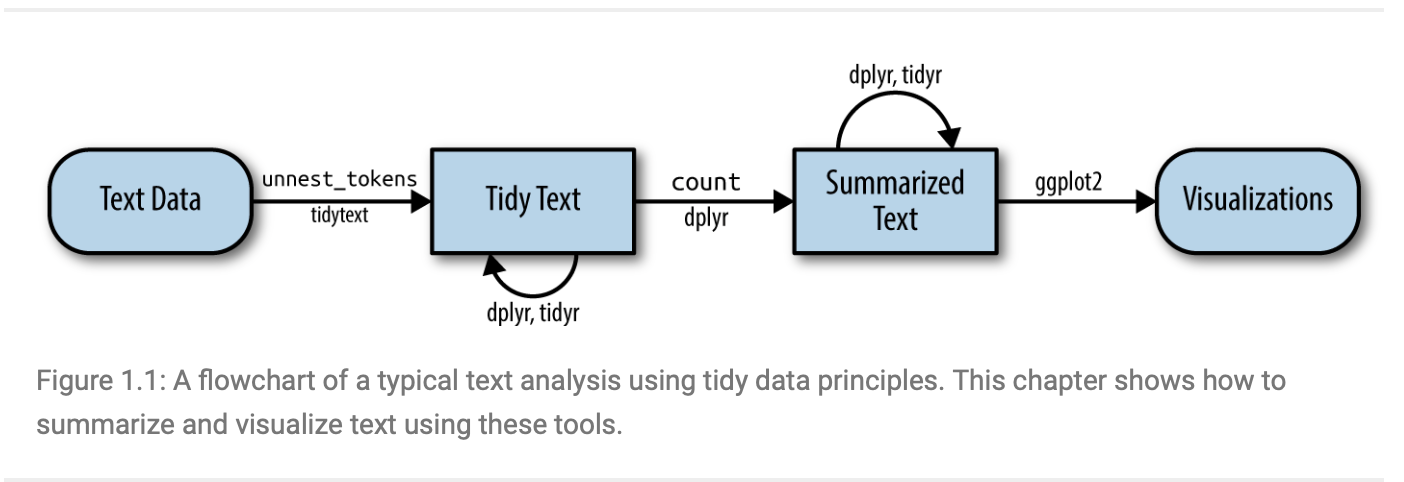
\includegraphics{Images/2.png}

\hypertarget{a-corpus}{%
\subsection{A Corpus}\label{a-corpus}}

For our analysis we need text. The raw text is the corpus that we work
on. The corpus that we are interested in varies depending on our
research objectives. For example, a corpus can contain a newspaper
articles, multiple articles, paragraphs from articles, tweets about a
particular topic or from a group of people, text from pdf documents that
we have collected etc. How we put together the relevant corpus depends
on the objective of our analysis.

Today we will work with some data that has already been provided to us.
The first is text from newspaper articles that were previously scraped
and the paragraphs collected into a dataframe.

The first step is to load the data. It was saved as an R Object, so we
can load it the following way:

\begin{Shaded}
\begin{Highlighting}[]
\FunctionTok{load}\NormalTok{(}\StringTok{"multiple\_url\_paragraphs.RData"}\NormalTok{)}
\end{Highlighting}
\end{Shaded}

This loads the R data object into our working environment to allow us to
begin working with the data. As you can see, it's loaded as, multi\_df.

The multi\_df data consists of a number of newspaper paragraphs
collected from the web and an id that identifies the number of the
paragraph in a given article. The id numbers repeat for each
article-paragraph.

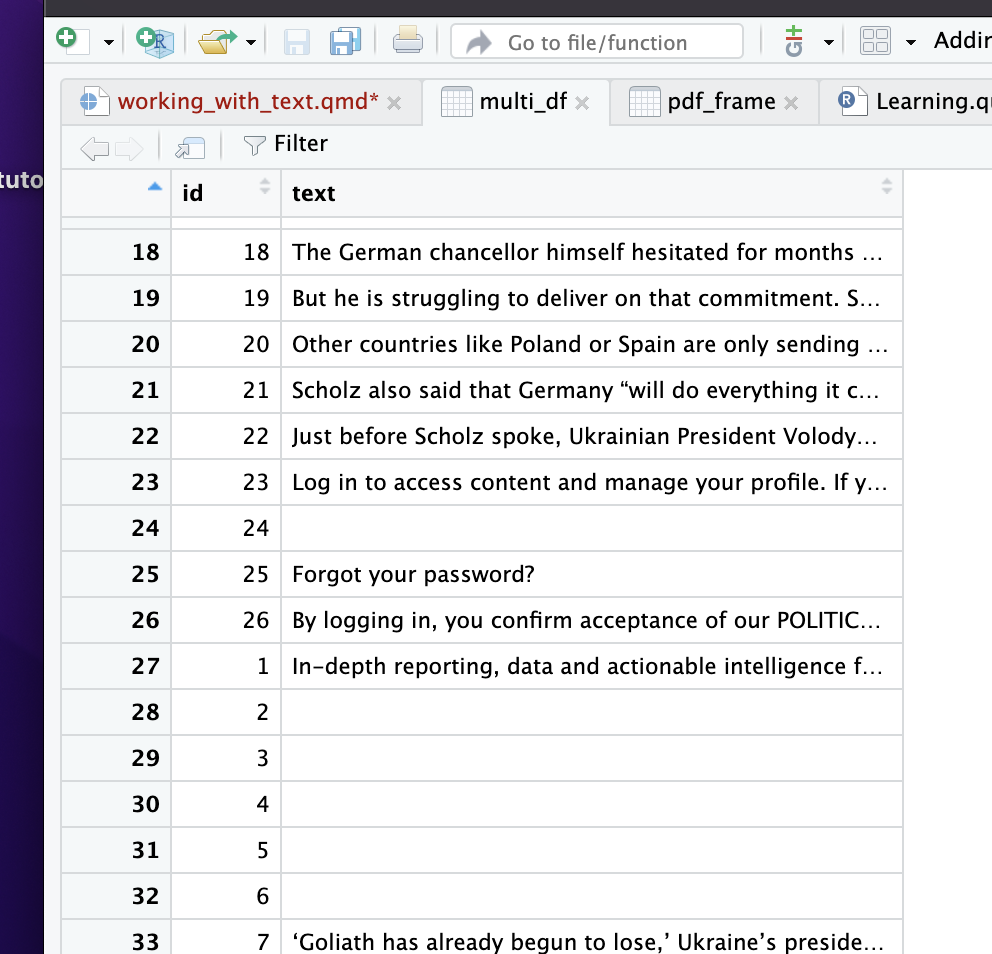
\includegraphics{Images/7.png}

\hypertarget{tokenization}{%
\section{Tokenization}\label{tokenization}}

To work with the unmodified corpus data we need to render it into a
format that we can use for text analysis. Specifically, the data we need
to turn it into a tokenized cleaned dataframe.

For this tutorial, we will be using the tidyverse text analysis method
because it is very intuitive so begin by loading the tidytext package
and installing it if not installed yet. This will be one of the core
packages needed for our work.

\begin{Shaded}
\begin{Highlighting}[]
\CommentTok{\# install.packages("tidytext")}
\FunctionTok{library}\NormalTok{(tidytext)}
\end{Highlighting}
\end{Shaded}

Now we can begin to work with the data.

First we want to transform the corpus into something more usable usable
by tokenizing the text.

By tokenizing the corpus we are separating the paragraphs and sentences
into words instead of the format they are currently in.

\begin{Shaded}
\begin{Highlighting}[]
\NormalTok{tidy\_paragraphs }\OtherTok{\textless{}{-}}\NormalTok{ multi\_df }\SpecialCharTok{\%\textgreater{}\%}
  \FunctionTok{unnest\_tokens}\NormalTok{(word, text)}
\end{Highlighting}
\end{Shaded}

If we look at tidy\_paragraphs, we can see that the text is broken down
by word and noted by the paragraph it is found in. The paragraph id
repeats for each article-paragraph-word that we downloaded that contains
text.

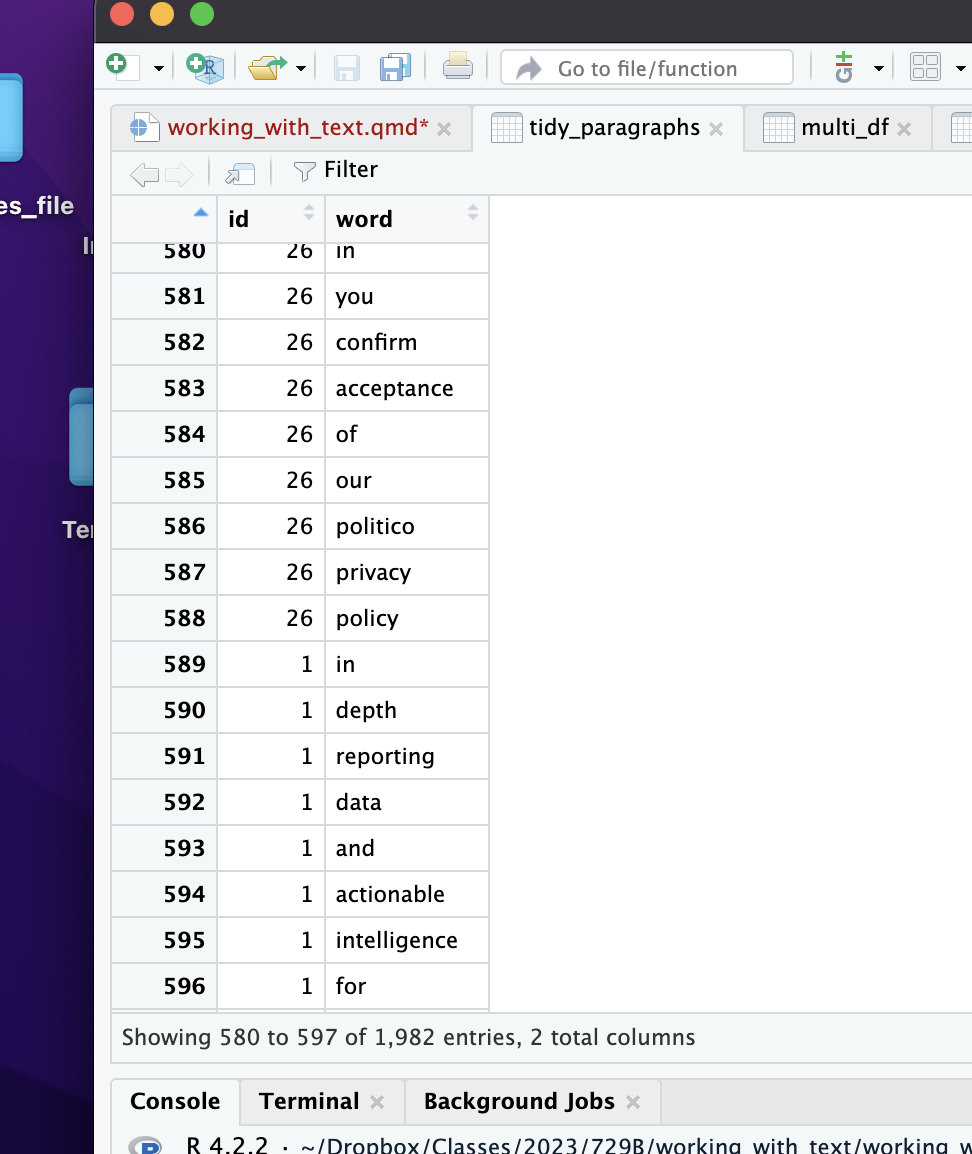
\includegraphics{Images/1.png}

\hypertarget{cleaning}{%
\subsubsection{Cleaning}\label{cleaning}}

Now we want to begin cleaning the corpus by removing unnecessary words.
These are words that convey no meaningful information but appear
frequently, usually referred to as ``stop words'' such as but, and, if,
then, and similar words.

\begin{Shaded}
\begin{Highlighting}[]
\NormalTok{tidy\_paragraphs }\OtherTok{\textless{}{-}}\NormalTok{ tidy\_paragraphs }\SpecialCharTok{\%\textgreater{}\%}
  \FunctionTok{anti\_join}\NormalTok{(stop\_words)}
\end{Highlighting}
\end{Shaded}

\begin{verbatim}
Joining with `by = join_by(word)`
\end{verbatim}

This uses the ``stop words'' dataset from tidyverse to remove the most
common stop words.

We can then look at the top words in our articles using the following
function:

\begin{Shaded}
\begin{Highlighting}[]
\NormalTok{tidy\_paragraphs }\SpecialCharTok{\%\textgreater{}\%}
  \FunctionTok{count}\NormalTok{(word, }\AttributeTok{sort =} \ConstantTok{TRUE}\NormalTok{) }
\end{Highlighting}
\end{Shaded}

This shows that the top words in these articles, with stop words
removed, are Munich, western, Ukraine, war, countries, and Germany.

You can also clean words/spaces/numbers that aren't stop words. This can
be especially useful if you accidentally include advertisements or other
unnecessary data in your scraping.

\begin{Shaded}
\begin{Highlighting}[]
\NormalTok{tidy\_paragraphs }\OtherTok{\textless{}{-}}\NormalTok{tidy\_paragraphs }\SpecialCharTok{\%\textgreater{}\%}
  \FunctionTok{filter}\NormalTok{(}\SpecialCharTok{!}\NormalTok{word }\SpecialCharTok{\%in\%} \FunctionTok{c}\NormalTok{(}\StringTok{"Politico"}\NormalTok{,}\StringTok{"reporting"}\NormalTok{)) }\CommentTok{\#Add in the word you\textquotesingle{}d like to remove here to filter them out}
\end{Highlighting}
\end{Shaded}

You can also clean out any numbers with the following code.

\begin{Shaded}
\begin{Highlighting}[]
\NormalTok{tidy\_paragraphs }\OtherTok{\textless{}{-}}\NormalTok{tidy\_paragraphs }\SpecialCharTok{\%\textgreater{}\%}
          \FunctionTok{filter}\NormalTok{(}\SpecialCharTok{!}\FunctionTok{grepl}\NormalTok{(}\StringTok{"[0{-}9]+"}\NormalTok{, word)) }
\CommentTok{\#filters out non{-}grepl (string) digits from 0{-}9 in any form in the word column}
\end{Highlighting}
\end{Shaded}

Cleaning is a lengthy and involved process that differs between every
project and depends on the data you are using. Take your time cleaning
the data to get the best results.

\hypertarget{analyzing-the-data}{%
\section{Analyzing the Data}\label{analyzing-the-data}}

Next we want to analyze the data.

\hypertarget{wordcloud-visualization}{%
\subsection{Wordcloud Visualization}\label{wordcloud-visualization}}

One common way to analyze the data is to visualize them.

For example, the most commonly used words can be visualized using a word
cloud. Two packages, devtools and wordcloud2, are needed to do this.

\begin{Shaded}
\begin{Highlighting}[]
\FunctionTok{library}\NormalTok{(wordcloud2)}
\FunctionTok{library}\NormalTok{(devtools)}
\end{Highlighting}
\end{Shaded}

\begin{verbatim}
Loading required package: usethis
\end{verbatim}

A wordcloud displays the words in the corpus by size according to how
often the words occur in the corpus. To show this we first must count
the words.

Words that occur more frequently will be larger and the ones that occur
less frequently will be smaller.

\begin{Shaded}
\begin{Highlighting}[]
\NormalTok{t\_para }\OtherTok{\textless{}{-}}\NormalTok{ tidy\_paragraphs }\SpecialCharTok{\%\textgreater{}\%}
  \FunctionTok{count}\NormalTok{(word, }\AttributeTok{sort =} \ConstantTok{TRUE}\NormalTok{) }
\end{Highlighting}
\end{Shaded}

Note that the new object (t\_para) counts words in the entire tokenized
corpus we fed to it (tidy\_paragraphs) and did NOT treat each
paragraph/article as a separate entity. You can make a very simple
wordcloud using the wordcloud2() function.

\begin{Shaded}
\begin{Highlighting}[]
\FunctionTok{wordcloud2}\NormalTok{(t\_para)}
\end{Highlighting}
\end{Shaded}

This then outputs a simple wordcloud of the most commonly use words in
our articles.

\hypertarget{word-sequences-n-grams}{%
\subsection{Word sequences N-grams}\label{word-sequences-n-grams}}

Alternatively we may want to establish relationships between words. For
example, by seeing how often word X is followed by word Y, we can build
a model of the relationships between them.

To do this we go back to the un-tokenized corpus multi\_df.

We can then use the function unnest\_tokens as used earlier in order to
tokenize into consecutive sequences of words (as opposed to single
words), called n-grams.

We do this by adding the token = ``ngrams'' option to unnest\_tokens(),
and setting n to the number of words we wish to capture in each n-gram.
When we set n to 2, we are examining pairs of two consecutive words,
often called ``bigrams'':

\begin{Shaded}
\begin{Highlighting}[]
\NormalTok{tidy\_bigrams }\OtherTok{\textless{}{-}}\NormalTok{ multi\_df }\SpecialCharTok{\%\textgreater{}\%}
  \FunctionTok{unnest\_tokens}\NormalTok{(bigram, text, }\AttributeTok{token =} \StringTok{"ngrams"}\NormalTok{, }\AttributeTok{n =} \DecValTok{2}\NormalTok{) }\SpecialCharTok{\%\textgreater{}\%}
  \FunctionTok{filter}\NormalTok{(}\SpecialCharTok{!}\FunctionTok{is.na}\NormalTok{(bigram)) }\CommentTok{\#NOTE here we are filtering out any words that are not a part of a bigram}
\end{Highlighting}
\end{Shaded}

Our usual tidy tools apply equally well to n-gram analysis. We can
examine the most common bigrams using dplyr's count():

\begin{Shaded}
\begin{Highlighting}[]
\NormalTok{tidy\_bigrams }\SpecialCharTok{\%\textgreater{}\%}
  \FunctionTok{count}\NormalTok{(bigram, }\AttributeTok{sort =} \ConstantTok{TRUE}\NormalTok{)}
\end{Highlighting}
\end{Shaded}

It then shows the pairs of words that frequently appear together.
Looking at it, you can see that the words are often two stop words and
thus, uninteresting. We can clean the data in order to filter the stop
words and focus on the interesting text.

This is a useful time to use tidyr's separate(), which splits a column
into multiple based on a delimiter. This lets us separate it into two
columns, ``word1'' and ``word2'', at which point we can remove cases
(rows) where either is a stop-word.

\begin{Shaded}
\begin{Highlighting}[]
\FunctionTok{library}\NormalTok{(tidyr)}

\NormalTok{bigrams\_separated }\OtherTok{\textless{}{-}}\NormalTok{ tidy\_bigrams }\SpecialCharTok{\%\textgreater{}\%}
  \FunctionTok{separate}\NormalTok{(bigram, }\FunctionTok{c}\NormalTok{(}\StringTok{"word1"}\NormalTok{, }\StringTok{"word2"}\NormalTok{), }\AttributeTok{sep =} \StringTok{" "}\NormalTok{)}

\NormalTok{bigrams\_filtered }\OtherTok{\textless{}{-}}\NormalTok{ bigrams\_separated }\SpecialCharTok{\%\textgreater{}\%}
  \FunctionTok{filter}\NormalTok{(}\SpecialCharTok{!}\NormalTok{word1 }\SpecialCharTok{\%in\%}\NormalTok{ stop\_words}\SpecialCharTok{$}\NormalTok{word) }\SpecialCharTok{\%\textgreater{}\%}
  \FunctionTok{filter}\NormalTok{(}\SpecialCharTok{!}\NormalTok{word2 }\SpecialCharTok{\%in\%}\NormalTok{ stop\_words}\SpecialCharTok{$}\NormalTok{word)}

\CommentTok{\# new bigram counts:}
\NormalTok{bigram\_counts }\OtherTok{\textless{}{-}}\NormalTok{ bigrams\_filtered }\SpecialCharTok{\%\textgreater{}\%} 
  \FunctionTok{count}\NormalTok{(word1, word2, }\AttributeTok{sort =} \ConstantTok{TRUE}\NormalTok{)}
\end{Highlighting}
\end{Shaded}

Now we can see the more interesting results:

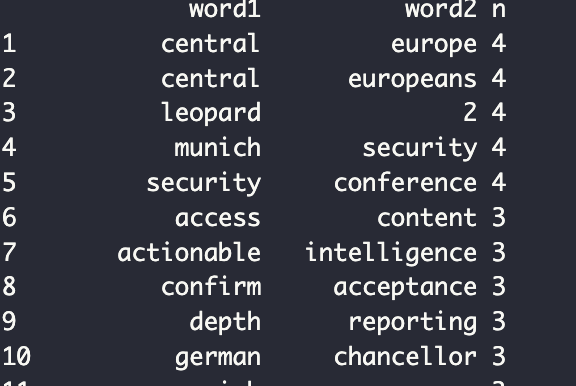
\includegraphics{Images/4.png}

\hypertarget{sentiment-analysis}{%
\subsection{Sentiment Analysis}\label{sentiment-analysis}}

When human readers approach a text, we use our understanding of the
emotional intent of words to infer whether a section of text is positive
or negative, or perhaps characterized by some other more nuanced emotion
like surprise or disgust. We can use the tools of text mining to
approach the emotional content of text programmatically, as shown below:

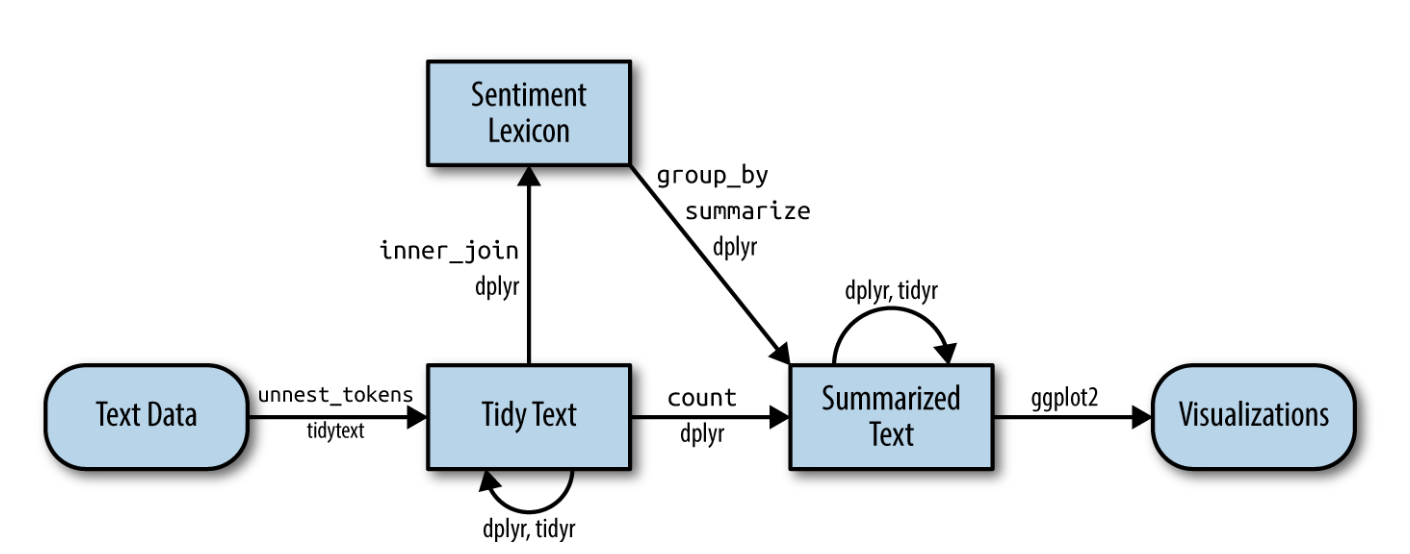
\includegraphics{Images/5.png}

There already exist quite a few existing dictionaries and methods for
sentiment analysis that make our work easier. The tidytext package
provides access to several ready made sentiment lexicons.

All three of these lexicons are based on unigrams, i.e., single words.
These lexicons contain many English words and the words are assigned
scores for positive/negative sentiment, and also possibly emotions like
joy, anger, or sadness.

The function get\_sentiments() allows us to get specific sentiment
lexicons with the appropriate measures for each one.

The following code is an example of how to use an existing sentiment
dictionary to analyze the text we worked with earlier. In order to make
the analysis more interesting, we can separate the analysis by document.
To do this, we will use data scraped from some pdf files.

\begin{Shaded}
\begin{Highlighting}[]
\FunctionTok{load}\NormalTok{(}\StringTok{"pdf\_frame1.RData"}\NormalTok{)}

\NormalTok{pdf\_frame1}\OtherTok{=}\NormalTok{pdf\_frame1}\SpecialCharTok{\%\textgreater{}\%}
  \FunctionTok{select}\NormalTok{(}\StringTok{"document"}\NormalTok{, }\StringTok{"term"}\NormalTok{)}
\end{Highlighting}
\end{Shaded}

Looking at this dataframe you see that it contains 2 column 1 for the
document number, one for the document-word.

First, rename the ``term'' column in pdf\_frame1 to word so it's easier
to join with the sentiment dictionary.

\begin{Shaded}
\begin{Highlighting}[]
\FunctionTok{colnames}\NormalTok{(pdf\_frame1)[}\DecValTok{2}\NormalTok{] }\OtherTok{=}\StringTok{"word"}
\end{Highlighting}
\end{Shaded}

Now, run this code to join the sentiment dictionary with the scraped
text and derive a sentiment score. This uses the ``bing'' sentiment
dictionary, which comes with the tidyverse packages:

\begin{Shaded}
\begin{Highlighting}[]
\NormalTok{multi\_doc\_sentiment }\OtherTok{\textless{}{-}}\NormalTok{ pdf\_frame1 }\SpecialCharTok{\%\textgreater{}\%}
  \FunctionTok{inner\_join}\NormalTok{(}\FunctionTok{get\_sentiments}\NormalTok{(}\StringTok{"bing"}\NormalTok{), }\AttributeTok{by=}\StringTok{"word"}\NormalTok{) }\SpecialCharTok{\%\textgreater{}\%}
  \FunctionTok{count}\NormalTok{(document, sentiment) }\SpecialCharTok{\%\textgreater{}\%}
  \FunctionTok{pivot\_wider}\NormalTok{(}\AttributeTok{names\_from =}\NormalTok{ sentiment, }\AttributeTok{values\_from =}\NormalTok{ n, }\AttributeTok{values\_fill =} \DecValTok{0}\NormalTok{) }\SpecialCharTok{\%\textgreater{}\%} 
  \FunctionTok{mutate}\NormalTok{(}\AttributeTok{sentiment =}\NormalTok{ positive }\SpecialCharTok{{-}}\NormalTok{ negative)}
\end{Highlighting}
\end{Shaded}

Note count(document, sentiment) asks the program to count sentiment
words by document and not in the whole corpus. This is useful for
comparing one document to the next.

Then the overall sentiment of the document is counted (positive
vs.~negative words)

Now we can compare the overall sentiments between documents data in the
, just as an example of what you can do with sentiment analysis. This
can be done via ggplot2.

\begin{Shaded}
\begin{Highlighting}[]
\FunctionTok{library}\NormalTok{(ggplot2)}

\NormalTok{p2 }\OtherTok{\textless{}{-}} \FunctionTok{ggplot}\NormalTok{(multi\_doc\_sentiment, }\FunctionTok{aes}\NormalTok{(document, sentiment, }\AttributeTok{fill =}\NormalTok{ document)) }\SpecialCharTok{+}
  \FunctionTok{geom\_col}\NormalTok{(}\AttributeTok{show.legend =} \ConstantTok{FALSE}\NormalTok{) }\SpecialCharTok{+}
  \FunctionTok{facet\_wrap}\NormalTok{(}\SpecialCharTok{\textasciitilde{}}\NormalTok{document, }\AttributeTok{ncol =} \DecValTok{2}\NormalTok{, }\AttributeTok{scales =} \StringTok{"free\_x"}\NormalTok{)}
\end{Highlighting}
\end{Shaded}

\begin{Shaded}
\begin{Highlighting}[]
\NormalTok{p2}
\end{Highlighting}
\end{Shaded}

\begin{figure}[H]

{\centering 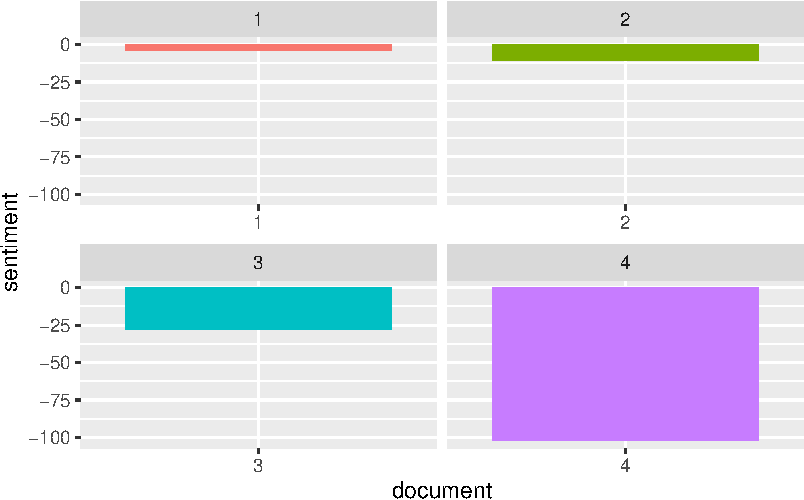
\includegraphics{working_with_text1_files/figure-pdf/unnamed-chunk-19-1.pdf}

}

\end{figure}

As shown in these graphs, document 4 is significantly more negative in
sentiment than the other three documents.

This is not altogether surprising as the first 3 documents are judicial
opinions whereas the 4th document is a Security council statement on the
situation in the Yugoslav republic.

\hypertarget{other-packages-and-options}{%
\section{Other packages and options}\label{other-packages-and-options}}

Text analysis has gained significant steam and multiple packages have
been developed to analyze sentiment and other features of text. Some of
the interesting and popular packages out there include:
\href{http://quanteda.io/}{Quanteda},
\href{https://cran.r-project.org/web/packages/tm/vignettes/tm.pdf}{Tm}
and many others. Some, including quanteda are discussed in the book we
based this tutorial largely on
\href{https://www.tidytextmining.com/index.html}{\textbf{Text Mining
with R}}, some are general purpose others satisfy a specific
requirement. We encourage you to read more if you are interested in
exploring this further.

Furthermore, when you develop your own research you may want to develop
your own dictionary for text depending on what you are looking for. For
example, the AMAR project (see ilcss) developed dictionaries to detect
ethnic minority groups and a variety of activity they engage in in news
paper text. We will learn more about this March 7th.

\hypertarget{assignment}{%
\section{Assignment}\label{assignment}}

Use the news data provided on github (or another corpus of your
choosing) to tokenize this corpus and clean of stopwords to produce a
graphical representation (word frequency, wordcloud etc.). Upload to
ELMS.



\end{document}
